%%%% Proceedings format for most of ACM conferences (with the exceptions listed below) and all ICPS volumes.
\documentclass[sigconf]{acmart}
%%%% As of March 2017, [siggraph] is no longer used. Please use sigconf (above) for SIGGRAPH conferences.

%%%% Proceedings format for SIGPLAN conferences 
% \documentclass[sigplan, anonymous, review]{acmart}

%%%% Proceedings format for SIGCHI conferences
% \documentclass[sigchi, review]{acmart}

%%%% To use the SIGCHI extended abstract template, please visit
% https://www.overleaf.com/read/zzzfqvkmrfzn

\usepackage{booktabs} % For formal tables
\usepackage[utf8]{inputenc}

% Copyright
\setcopyright{othergov}
%\setcopyright{acmcopyright}
%\setcopyright{acmlicensed}
%\setcopyright{rightsretained}
%\setcopyright{usgov}
%\setcopyright{usgovmixed}
%\setcopyright{cagov}
%\setcopyright{cagovmixed}

\begin{document}
\title{Uma Revisão Sistemática sobre o uso das Metodologias Ágeis}  
\author{F.C.A Dias}
\affiliation{%
  \institution{University of São Paulo}
}
\email{felipecavazotto@usp.br}

% \begin{abstract}
% This paper provides a sample of a \LaTeX\ document which conforms,
% somewhat loosely, to the formatting guidelines for
% ACM SIG Proceedings.\footnote{This is an abstract footnote}
% \end{abstract}

\maketitle

\section{Introdução}
O Manifesto Ágil \cite{Beck2001}, inicia-se dizendo haver mais valor nas interações entre indivíduos, em códigos de software legíveis, na colaboração com os clientes e na capacidade de se responder a mudanças do que em processos e ferramentas, documentação e planos pré-estabelecidos. Com base nisso, foram formulados doze princípios (P1 a P12) direcionando o desenvolvimento de software a ser adaptativo e orientado a pessoas \cite{Beck2001}: \newline

P1- Nossa maior prioridade é satisfazer o cliente através da entrega contínua e adiantada de software com valor agregado.

P2 - Mudanças nos requisitos são bem-vindas, mesmo tardiamente no desenvolvimento. Processos ágeis tiram vantagem das 
mudanças visando vantagem competitiva para o cliente.

P3 - Entregar frequentemente software funcionando, de poucas semanas a poucos meses, com preferência à menor escala de tempo.

P4 - Pessoas de negócio e desenvolvedores devem trabalhar diariamente em conjunto por todo o projeto.

P5 - Construa projetos em torno de indivíduos motivados. Dê a eles o ambiente e o suporte necessário e confie neles para fazer o trabalho.

P6 - O método mais eficiente e eficaz de transmitir informações para e entre uma equipe de desenvolvimento é através de conversa face a face.

P7 - Software funcionando é a medida primária de progresso.

P8 - Os processos ágeis promovem desenvolvimento sustentável. Os patrocinadores, desenvolvedores e usuários devem ser capazes de manter um ritmo constante indefinidamente.

P9 - Contínua atenção à excelência técnica e bom design aumenta a agilidade.

P10 - Simplicidade -- a arte de maximizar a quantidade de trabalho não realizado -- é essencial.

P11 - As melhores arquiteturas, requisitos e designs emergem de equipes auto-organizáveis.

P12 - Em intervalos regulares, a equipe reflete sobre como se tornar mais eficaz e então refina e ajusta seu comportamento de acordo. \newline

Apesar da simplicidade desses conceitos, eles assim como outros que se popularizam, passam por um processo de Difusão Semântica \cite{sematicDiffusion}, no qual pode ocorrer perda dos valores inicialmente estabelecidos a medida em que são internalizados pelas pessoas. Trata-se de um ciclo cognitivo natural do aprendizado, sujeito ao consenso e amadurecimento  da Indústria de Software. Devido a isso, inúmeros fatores podem impactar no uso das Metodologias Ágeis.

\section{Metodologia}

A presente Revisão Sistemática utiliza a metodologia proposta por \citeauthor{biolchini2005techincal} \citeyear{biolchini2005techincal}, composta por cinco etapas.
A primeira etapa está relacionada à formulação do problema, na qual é levantada uma questão central se referindo ao tipo de evidência que deverá  estar contida na revisão \citeauthor{biolchini2005techincal} \citeyear{biolchini2005techincal}. Em seguida, são construídas definições que permitam estabelecer distinção entre os estudos relevantes e irrelevantes para o propósito específico do que se está investigando \citeauthor{biolchini2005techincal} \citeyear{biolchini2005techincal}.

A segunda etapa da condução está relacionada à Coleta de Dados, na qual são definidos os procedimentos que serão utilizados para encontrar a evidência relevante que foi definida na etapa anterior \citeauthor{biolchini2005techincal} \citeyear{biolchini2005techincal}. Nesta fase é extremamente importante determinar as fontes que podem fornecer estudos relevantes a serem incluídos na pesquisa \citeauthor{biolchini2005techincal} \citeyear{biolchini2005techincal}.

Na terceira etapa, defini-se a Avaliação de Dados, na qual são selecionados as fontes primárias que deverão ser incluídas na revisão \citeauthor{biolchini2005techincal} \citeyear{biolchini2005techincal}. Em seguida,  são aplicados os critérios de qualidade para separar estudos que podem ser considerados válidos, e determinadas as diretrizes para o tipo de informação que deve ser extraída dos relatórios de pesquisas primárias \citeauthor{biolchini2005techincal} \citeyear{biolchini2005techincal}.

A quarta etapa da revisão é o processo de Análise e Interpretação, na qual os dados dos estudos primários válidos são sintetizados \citeauthor{biolchini2005techincal} \citeyear{biolchini2005techincal}. E, na quinta etapa são realizados os processos de Conclusão e Apresentação \citeauthor{biolchini2005techincal} \citeyear{biolchini2005techincal}.

\subsection{Formulação do Problema}
Os princípios do Manifesto Ágil \cite{Beck2001}, assim como qualquer outro conceito, passam por um processo de Difusão Semântica, sendo afetado por inúmeros fatores,  segundo \citeauthor{sematicDiffusion} \citeyear{sematicDiffusion}. Nesse contexto, a seguinte questão de pesquisa foi formulada: \newline

QP1 - Quais fatores têm impactado no uso das Metodologias Ágeis nos últimos cinco anos? \newline

\subsection{Coleta de Dados}
Nesta Revisão Sistemática, os artigos foram coletados em quatro fontes de pesquisa, por meio da plataforma de indexação de trabalhos acadêmicos Google Scholar. Constam na Tab. \ref{tab:tableNumberOfArticles} as bases pesquisadas, quantidades de artigos coletados, descartados no processo de filtragem (Fig. \ref{fig:filter}) e selecionados. Com base na QP1, a seguinte \textit{string} de busca foi construída; restrita aos trabalhos publicados entre 2011 e 2016, escritos no idioma Inglês: \newline \newline (USAGE OF AGILE) AND \newline (AGILE OR SOFTWARE OR DEVELOPMENT).

\begin{table}[!htb]
\centering
\caption{Quantidades de artigos coletados e fontes de busca}
	\label{tab:tableNumberOfArticles}
\begin{tabular}{c|c|c|c}
\hline
{\bf Fonte} & \bf {Artigos coletados} & {\bf Filtragem} & {\bf Selecionados}\\ 
\hline
ACM & 13 & 11 & 2 \\ 
\hline
IEEE & 35 & 28 & 7 \\ 
\hline
Elsevier & 14 & 12 & 2\\ 
\hline
Springer & 25 & 19 & 6\\ 
\hline
{-} & 87 & 70 & 17\\ 
\hline
\end{tabular}
\center{\bf Fonte:} Felipe Dias
\end{table}

\begin{figure}
\centering
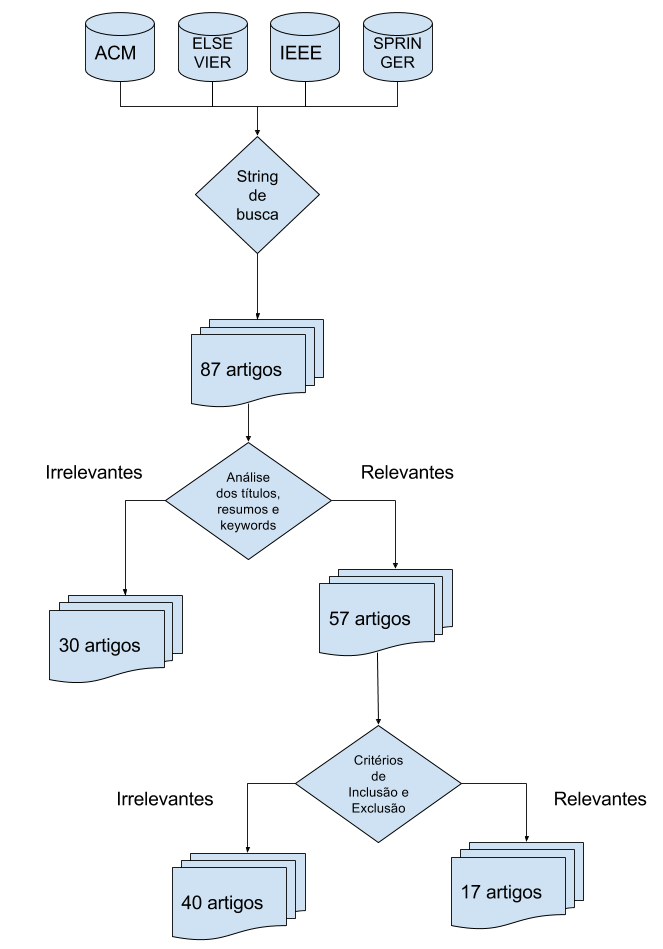
\includegraphics[width=1\linewidth]{metodologia_gestao.png}
\caption{Processo de Filtragem}
\center{\bf Fonte:} Felipe Dias
\label{fig:filter}
\end{figure}

\subsection{Avaliação de Dados}

Visando selecionar os artigos relevantes para esta Revisão Sistemática, os seguintes critérios foram utilizados:

\begin{itemize}
\item Trabalho publicado.
\item Trabalhos que abordam o uso de metodologias ágeis num contexto genérico.
\item Trabalhos duplicados.
\item Trabalhos que estão fora do escopo da questão de pesquisa (Metodologias Ágeis).
\end{itemize}

O processo de condução da Revisão Sistemática foi realizado utilizando os critérios acima mencionados, e está disponível em \cite{fcas}.

\section{Análise e Interpretação}

\citeauthor{Senapathi2012} \citeyear{Senapathi2012} propuseram um modelo contendo os seguintes fatores que impactam no uso das Metodologias Ágeis: Fatores relacionados a Inovação , Sociológicos, Tecnológicos e Organizacionais, divididos em algumas categorias, que não serão detalhadas nesse trabalho. Nessa modelagem, há uma relação bidirecional entre uso e eficácia das Metodologias Ágeis na Produtividade, Qualidade e Satisfação do Cliente.

Os textos coletados foram separados nas categorias mencionadas anteriormente, desconsiderando as subcategorias e a relação bidirecional proposta originalmente por \citeauthor{Senapathi2012} \citeyear{Senapathi2012}.

\subsection{Fatores tecnológicos}

Segundo \citeauthor{Senapathi2014} \citeyear{Senapathi2014}, a adoção de ferramentas adequadas afeta o uso das Metodologias Ágeis, em termos de suporte a práticas específicas, tais como refatoração, integração contínua e desenvolvimento orientado a teste. Tais ferramentas, precisam ser fáceis de usar, otimizáveis, integráveis a outras ferramentas e personalizáveis \citeauthor{Azizyan2011} \citeyear{Azizyan2011}. No entanto, em \citeauthor{Asnawi2011} \citeyear{Asnawi2011}, afirma-se que outros fatores como os sociológicos podem ser mais relevantes que os tecnológicos. Além disso, ressaltam a importância das ferramentas relacionadas a comunicação entre os times, pois na ausência de informação, a tendência é a de assumir a interpretação de determinado requisito do ponto de vista da pessoa responsável por ele.

\subsection{Fatores relacionados a inovação}

\citeauthor{Senapathi2011} \citeyear{Senapathi2011} e \citeauthor{Senapathi2012} \citeyear{Senapathi2012} citam que a difusão da inovação é um processo de seis etapas, incluindo iniciação (reconhecimento de que alguma mudança é necessária), adoção (tomada de decisão para adotar determinada inovação), adaptação (as necessidades contextuais), aceitação (uso da inovação), rotina (aumento da extensão e intensidade do uso) e infusão (incorporação da inovação); sendo as três fases iniciais relacionadas ao processo adotivo, e as três últimas ao uso pós-adotivo de uma inovação.

Assim, \citeauthor{Senapathi2011} \citeyear{Senapathi2011} e \citeauthor{Senapathi2012} \citeyear{Senapathi2012} argumentam que o estágio do processo pós-adotivo somente é alcançado quando a inovação oferece melhorias específicas em relação ao sua antecessora (fatores relacionados a percepção de utilidade e facilidade de uso, apontados por \citeauthor{Bahli2011} \citeyear{Bahli2011}, no contexto da absorção de conceitos). Ou seja, o uso das Metodologias Ágeis está relacionado as suas respectivas vantagens oferecidas \citeauthor{Senapathi2011} \citeyear{Senapathi2011} e \citeauthor{Senapathi2012} \citeyear{Senapathi2012}.

\subsection{Fatores organizacionais}
De acordo com \citeauthor{Senapathi2014} \citeyear{Senapathi2014}, as Metodologias Ágeis precisam ser compatíveis ao contexto no qual estão inseridas, devido ao fato de demandarem modificações importantes no modo de trabalho, na adoção de ferramentas que facilitam o desenvolvimento ágil iterativo, gerenciamento do controle de versão e configuração, refatoração, dentre outras práticas. Tal processo pode demandar treinamento de funcionários \citeauthor{Lazwanthi2016} \citeyear{Lazwanthi2016}, \citeauthor{Pikkarainen2012} \citeyear{Pikkarainen2012} e \citeauthor{Solinski2016} \citeyear{Solinski2016}.

Além disso, \citeauthor{Senapathi2012} \citeyear{Senapathi2012}, \citeyear{Senapathi2014}; \citeauthor{Asnawi2012} \citeyear{Asnawi2012}, \citeauthor{Pikkarainen2012} \citeyear{Pikkarainen2012} e \citeauthor{Solinski2016} \citeyear{Solinski2016}, afirmam que é necessário apoio contínuo e envolvimento direto por parte da alta gestão, incentivando o uso, implementação de inovações, determinados comportamentos, atuando como um fator crítico na difusão das Metodologias Ágeis; assim como a presença de facilitadores, que por meio de influências sociais e políticas ajudam a eliminar barreiras existentes na organização.

Nesse contexto, a cultura e estrutura da organização também exercem influência considerável sobre o uso das Metodologias Ágeis, afirmam \citeauthor{Asnawi2012} \citeyear{Asnawi2012}, \citeauthor{Senapathi2014} \citeyear{Senapathi2014}, \citeauthor{Lazwanthi2016} \citeyear{Lazwanthi2016}, \citeauthor{B2016} \citeyear{B2016}, \citeauthor{Laanti2011} \citeyear{Laanti2011}. Apesar disso, segundo \citeauthor{Lazwanthi2016} \citeyear{Lazwanthi2016} e \citeauthor{Asnawi2012} \citeyear{Asnawi2012}, inúmeras empresas se adaptam à cultura ágil devido aos seus benefícios, tais como melhoria do relacionamento com o cliente (\citeauthor{Solinski2016} \citeyear{Solinski2016}), resultados mensuráveis a curto prazo, melhor comunicação (\citeauthor{Murphy2013} \citeyear{Murphy2013}), conhecimento das atividades por todos (\citeauthor{Murphy2013} \citeyear{Murphy2013}), pouco foco em documentação, retrospectiva, integração contínua, \textit{standup meetings}, aumento da colaboração (\citeauthor{B2016} \citeyear{B2016}), \textit{feedbacks} e qualidade (\citeauthor{Solinski2016} \citeyear{Solinski2016} e \citeauthor{Murphy2013} \citeyear{Murphy2013}), dentre outros. Tais benefícios normalmente são alcançados a longo prazo devido a demora na adoção de muitas das práticas, situação que pode estar relacionada ao nível de experiência das partes envolvidas \citeauthor{B2016} \citeyear{B2016}. 

Tal velocidade é normal ante aos desafios impostos pela transição entre os métodos tradicionais e ágeis, segundo \citeauthor{Lazwanthi2016} \citeyear{Lazwanthi2016}, \citeauthor{B2016} \citeyear{B2016}, \citeauthor{Laanti2011} \citeyear{Laanti2011}. Entre os desafios, destacam-se a ausência de documentação (exigida por alguns clientes; e para transferência de conhecimento \citeauthor{Asnawi2011} \citeyear{Asnawi2011}), escalabilidade (\citeauthor{Solinski2016} \citeyear{Solinski2016}), esforço demandado para o desenvolvimento de testes (\citeauthor{Solinski2016} \citeyear{Solinski2016}), excesso de \textit{standup meetings} (\citeauthor{Murphy2013} \citeyear{Murphy2013}), resistências organizacionais, pessoais (como muito tempo de experiência com as metodologias tradicionais \citeauthor{Laanti2011} \citeyear{Laanti2011}, envolvimento entre as partes interessadas, conhecimento profundo sobre as Metodologias Ágeis (evitando uso errôneo \citeauthor{Murphy2013} \citeyear{Murphy2013}), culturais (regionais), governamentais e ausência de recursos (combinação de múltiplas responsabilidades - necessidade de diferentes responsabilidades a pessoas distintas) \citeauthor{Asnawi2012} \citeyear{Asnawi2012}.

No entanto, as organizações não necessariamente precisam mudar sua cultura atual para usar as Metodologias Ágeis \citeauthor{Bunyakiati2016} \citeyear{Bunyakiati2016}. Em vez disso, elas podem selecionar a prática ágil mais adequada ao seu tipo cultural. Neste mesmo posicionamento, \citeauthor{Lazwanthi2016} \citeyear{Lazwanthi2016}, menciona que para a implementação da cultura ágil seja bem-sucedida, é importante compreender as questões culturais relacionadas a cada metodologia \citeauthor{Lazwanthi2016} \citeyear{Lazwanthi2016}. Por exemplo, \citeauthor{Lazwanthi2016} \citeyear{Lazwanthi2016} defende que as práticas \textit{SCRUM} e \textit{eXtreme Programming (XP)} podem ser implementados somente em organizações de pequeno e médio porto, não sendo implementáveis como único método em uma organização globalmente distribuída, pois um dos fatores desafiadores está relacionado a sincronia entre os recursos em diferentes fusos horários, o que afirma também \citeauthor{Asnawi2012} \citeyear{Asnawi2011}, \citeyear{Asnawi2012}. As metodologias híbridas podem ser vistas como as mais compatíveis com a maioria das culturas organizacionais \citeauthor{Lazwanthi2016} \citeyear{Lazwanthi2016}, enquanto que as puramente ágeis com empresas pequenas \citeauthor{Asnawi2011} \citeyear{Asnawi2011}.

Nesse contexto, empresas que se concentram nas pessoas e na interação entre elas, tendem a adotar \textit{Scrum} e \textit{XP} como práticas ágeis; as focadas nas questões relacionadas ao software, optam por \textit{Behavior Development} (BDD), \textit{Test-Driven Development} (TDD) e \textit{Acceptance-Test-Driven Development} (ATDD); as direcionas ao domínio ao qual pertencem os problemas, pelo \textit{Dynamic System Development Metodoly} (DSDM) e \textit{Feature-driven Development} (FDD); e por fim, as que dão mais importância ao gerenciamento de fluxo e capacidade do processo de software, normalmente adotam as metodologias \textit{Lean Software Development} e \textit{Kanban}, segundo \citeauthor{Lazwanthi2016} \citeyear{Lazwanthi2016}. 

Apesar das diferentes escolhas de metodologias, \citeauthor{Diebold} \citeyear{Diebold} menciona que em torno de 52\% dos projetos usam técnicas de retrospectiva, 50\% planejamento iterativo e estórias de usuários, 48\% standup meetings, 40\% integração contínua, \textit{product owner} dedicado aos clientes e uso verificação e validação; menos de 40\% utilizam monitoramento de progresso (\textit{Kanban}, \textit{burndown chart}, \textit{backlog}), qualidade (programação em pares, teste unitários, TDD), bases de conhecimento e refatoração. No entanto, essas taxas de uso mudam de acordo com a função exercida pela pessoa, no estudo realizado em \citeauthor{Murphy2013} \citeyear{Murphy2013}, a porcentagem de uso de testes de aceitação foi maior em 10\%, na comparação entre testadores e desenvolvedores, sendo 14\% maior a probabilidade de uso por parte dos testadores; analogamente, a probabilidade dos gerentes de produto utilizarem retrospectivas, \textit{burndown charts}, estórias de usuário, contado direto com clientes e testes de aceitação é maior em mais de 10\% se comparada com a dos desenvolvedores; e estes por sua vez têm probabilidade em mais de 10\% para o uso de repositórios de código, em comparação aos demais.   

Independentemente das práticas, a liberdade das partes envolvidas para escolhê-la atua como fator de sucessos na adoção das Metodologias Ágeis \citeauthor{Pikkarainen2012} \citeyear{Pikkarainen2012}, assim como o uso do idioma Inglês \citeauthor{Asnawi2014} \citeyear{Asnawi2014}. Além disso, \citeauthor{Solinski2016} \citeyear{Solinski2016} mencionam que algumas práticas são abandonadas ao longo do tempo, tais com programação em pares, desenvolvimento dirigido a testes e integração contínua com testes. Observa-se também, a continuidade no uso das Metodologias Ágeis pela maioria das pessoas, existindo que algumas desistem de utilizá-las \citeauthor{Murphy2013} \citeyear{Murphy2013}.  

\subsection{Fatores sociológicos}

\citeauthor{Senapathi2014} \citeyear{Senapathi2014} menciona que a principal filosofia das Metodologias Ágeis se baseia na melhoria contínua (P1), a qual engloba características sociológicas, tais como atitude positiva, vontade de aprender e mudar, crença na equipe e espírito de equipe (senso de identificação e compromisso com a equipe, mesmo que haja opiniões diferentes); que se resumem no fator conhecido como mentalidade ágil. E, a aderência dos desenvolvedores a essa mentalidade ágil é um dos fatores cruciais capazes de influênciar o uso das Metodologias Ágeis, segundo \citeauthor{Asnawi2011} \citeyear{Asnawi2011}, \citeyear{Asnawi2012}.

Nesse cenário, \citeauthor{Senapathi2014} \citeyear{Senapathi2014} e \citeauthor{Solinski2016} \citeyear{Solinski2016}, afirmam que o auxílio de um \textit{coaching} pode ser utilizado nas fases iniciais de adoção e conscientização das Metodologias Ágeis, sendo um fator sociológico importante na criação e manutenção de equipes de desenvolvimento de software. Outros fatores sociológicos mencionados são os relacionados a atitude (crenças positivas ou negativas da equipe sobre as consequências de continuar a usar uma inovação) e experiência (uma equipe com um alto nível de especialização pode não estar sujeita à curva de aprendizado associada a um domínio desconhecido) \citeauthor{Senapathi2012} \citeyear{Senapathi2012}.

Além disso, \citeauthor{Senapathi2012} \citeyear{Senapathi2012} cita que níveis mais altos de atributos pessoais, como inovação, resiliência e tolerância de ambiguidade, podem facilitar a difusão das Metodologias Ágeis, enquanto que níveis mais baixos podem ser restritivos. \citeauthor{Laanti2013} \citeyear{Laanti2013}, adiciona que o princípio sobre o desenvolvimento sustentável (P8) pode ter impacto no fator sociológico relacionado ao sentimento de pressão para entregas constantes, influenciando no nível de estresse. Apesar de não haver significância estatística entre essa relação, estudos comprovam que o nível de estresse está relacionado a performance. \citeauthor{B2016} \citeyear{B2016} acharam surpreendente que as Metodologias Ágeis fossem capazes de estarem ligadas a fatores de estresse e excesso de trabalho, pois difundem filosofias de colaboração, auto-gerenciamento, pequenas interações, favoráveis ao bem estar, como confirmam \citeauthor{Solinski2016} \citeyear{Solinski2016} e \citeauthor{Kurapati2012} \citeyear{Kurapati2012}. No entanto, o contrário acontece devido a aspectos sociais, como o controle social e relação de compromisso com a equipe, sensação que é experimentada tanto por profissionais com pouca experiência quanto aos com muita \citeauthor{B2016} \citeyear{B2016}.

\section{Discussão}

\subsection{Fatores tecnológicos}

Os princípios do Manifesto Ágil \cite{Beck2001} não fazem menção a nenhum fator tecnológico, no entanto, algumas ferramentas facilitam uso de práticas relacionadas refatoração, integração contínua e desenvolvimento orientado a teste, assim como a comunicação entre os membros da equipe. Apesar disso, o princípio número seis  afirma que método mais eficiente e eficaz de transmitir informações para e entre uma equipe de desenvolvimento é através de conversa face a face \cite{Beck2001}. Além disso, a afirmação do princípio cinco suporta o argumento de que fatores sociológicos têm mais impacto do que os tecnológicos, dizendo que os projetos precisam ser construídos em torno de indivíduos motivados.

\subsection{Fatores relacionados a inovação}

Os estudos analisados argumentam que os fatores relacionados a inovação, focam em sua respectiva difusão e absorção. Sendo assim, no início desse processo, uma necessidade de mudança é percebida, seguindo pela tomada de decisão, adaptação, uso, aumento da intensidade de uso e incorporação da inovação. Nesse aspecto, o principio número dois do Manifesto Ágil é favorável a inovação, afirmando que os processos ágeis tiram vantagem das mudanças visando vantagem competitiva para o cliente \cite{Beck2001}. No entanto, o uso desse princípio pode ser ameaçado dependendo de como as empresas e pessoas envolvidas lidam com as inovações propostas por eles.

\subsection{Fatores organizacionais}
De acordo com os estudos analisados, todos os autores que abordam os fatores organizacionais, concordam que eles impactam no uso das Metodologias Ágeis. Impactando negativamente quando a cultura da organização não é compatível com os princípios do Manifesto Ágil, demandando assim modificações importantes no modo de trabalho. No entanto, isso pode não acontecer devido ao fato dessas empresas poderem optar por metodologias específicas que melhores se adequam as suas realidades, assim como criarem alternativas híbridas, aproveitando os benefícios de cada uma, deixando as desvantagens a parte, ou, simplesmente abandonando o uso de alguns princípios.

Além dos processos de adaptação, o princípio número quatro do Manifesto Ágil \cite{Beck2001}, afirma que as pessoas relacionadas ao negócio e os desenvolvedores devem trabalhar diariamente em conjunto. Nesse sentindo, os estudos analisados afirmam que é necessário apoio contínuo e envolvimento direto por parte da alta gestão e facilitadores, incentivando o uso das metodologias Ágeis.

\subsection{Fatores sociológicos}

De acordo com os estudos analisados, há consenso referente aos fatores sociológicos. Cada autor contribui com diferentes frentes, seja afirmando que atitudes que estão de acordo com o princípio de melhoria contínua favorecem o uso das Metodologias Ágeis, ou, sobre atributos pessoais atuando como restritivos, como é o caso da baixa resiliência. Apenas dois estudos mencionaram questões referentes ao desenvolvimento sustentável e sua relação com níveis de estresse e desempenho.

\section{Conclusão}

Nos últimos cinco anos, principalmente em 2011 e 2012, muitos estudos se concentraram em aspectos relacionados aos fatores organizacionais, mencionando as dificuldades que as empresas tiveram até de fato iniciarem o uso das metodologias ágeis. Estudos mais recentes tem focado em fatores sociológicos, pois a fase de transição do modo tradicional para o ágil, provavelmente já passou para a maioria das empresas.

\section{Limitações}

As limitações dessa Revisão Sistemática estão relacionadas a busca por estudos genéricos sobre o uso das Metodologias Ágeis e a não abordagem dos processos existentes no ciclo de desenvolvimento de software.

\section{Indicações de trabalhos futuros}
Como resultado do processo de Revisão Sistemática, foram encontrados poucos estudos relacionados aos fatores sociológicos envolvendo o uso das Metodologias Ágeis, sendo possivelmente um assunto a ser melhor explorado.

% Typically, the body of a paper is organized into a hierarchical
% structure, with numbered or unnumbered headings for sections,
% subsections, sub-subsections, and even smaller sections.  The command
% \texttt{{\char'134}section} that precedes this paragraph is part of
% such a hierarchy.\footnote{This is a footnote.} \LaTeX\ handles the
% numbering and placement of these headings for you, when you use the
% appropriate heading commands around the titles of the headings.  If
% you want a sub-subsection or smaller part to be unnumbered in your
% output, simply append an asterisk to the command name.  Examples of
% both numbered and unnumbered headings will appear throughout the
% balance of this sample document.

% Because the entire article is contained in the \textbf{document}
% environment, you can indicate the start of a new paragraph with a
% blank line in your input file; that is why this sentence forms a
% separate paragraph.

% \subsection{Type Changes and {\itshape Special} Characters}

% We have already seen several typeface changes in this sample.  You can
% indicate italicized words or phrases in your text with the command
% \texttt{{\char'134}textit}; emboldening with the command
% \texttt{{\char'134}textbf} and typewriter-style (for instance, for
% computer code) with \texttt{{\char'134}texttt}.  But remember, you do
% not have to indicate typestyle changes when such changes are part of
% the \textit{structural} elements of your article; for instance, the
% heading of this subsection will be in a sans serif\footnote{Another
%   footnote here.  Let's make this a rather long one to see how it
%   looks.} typeface, but that is handled by the document class file.
% Take care with the use of\footnote{Another footnote.}  the
% curly braces in typeface changes; they mark the beginning and end of
% the text that is to be in the different typeface.

% You can use whatever symbols, accented characters, or non-English
% characters you need anywhere in your document; you can find a complete
% list of what is available in the \textit{\LaTeX\ User's Guide}
% \cite{Lamport:LaTeX}.

% \subsection{Math Equations}
% You may want to display math equations in three distinct styles:
% inline, numbered or non-numbered display.  Each of
% the three are discussed in the next sections.

% \subsubsection{Inline (In-text) Equations}
% A formula that appears in the running text is called an
% inline or in-text formula.  It is produced by the
% \textbf{math} environment, which can be
% invoked with the usual \texttt{{\char'134}begin\,\ldots{\char'134}end}
% construction or with the short form \texttt{\$\,\ldots\$}. You
% can use any of the symbols and structures,
% from $\alpha$ to $\omega$, available in
% \LaTeX~\cite{Lamport:LaTeX}; this section will simply show a
% few examples of in-text equations in context. Notice how
% this equation:
% \begin{math}
%   \lim_{n\rightarrow \infty}x=0
% \end{math},
% set here in in-line math style, looks slightly different when
% set in display style.  (See next section).

% \subsubsection{Display Equations}
% A numbered display equation---one set off by vertical space from the
% text and centered horizontally---is produced by the \textbf{equation}
% environment. An unnumbered display equation is produced by the
% \textbf{displaymath} environment.

% Again, in either environment, you can use any of the symbols
% and structures available in \LaTeX\@; this section will just
% give a couple of examples of display equations in context.
% First, consider the equation, shown as an inline equation above:
% \begin{equation}
%   \lim_{n\rightarrow \infty}x=0
% \end{equation}
% Notice how it is formatted somewhat differently in
% the \textbf{displaymath}
% environment.  Now, we'll enter an unnumbered equation:
% \begin{displaymath}
%   \sum_{i=0}^{\infty} x + 1
% \end{displaymath}
% and follow it with another numbered equation:
% \begin{equation}
%   \sum_{i=0}^{\infty}x_i=\int_{0}^{\pi+2} f
% \end{equation}
% just to demonstrate \LaTeX's able handling of numbering.

% \subsection{Citations}
% Citations to articles~\cite{bowman:reasoning,
% clark:pct, braams:babel, herlihy:methodology},
% conference proceedings~\cite{clark:pct} or maybe
% books \cite{Lamport:LaTeX, salas:calculus} listed
% in the Bibliography section of your
% article will occur throughout the text of your article.
% You should use BibTeX to automatically produce this bibliography;
% you simply need to insert one of several citation commands with
% a key of the item cited in the proper location in
% the \texttt{.tex} file~\cite{Lamport:LaTeX}.
% The key is a short reference you invent to uniquely
% identify each work; in this sample document, the key is
% the first author's surname and a
% word from the title.  This identifying key is included
% with each item in the \texttt{.bib} file for your article.

% The details of the construction of the \texttt{.bib} file
% are beyond the scope of this sample document, but more
% information can be found in the \textit{Author's Guide},
% and exhaustive details in the \textit{\LaTeX\ User's
% Guide} by Lamport~\shortcite{Lamport:LaTeX}.


% This article shows only the plainest form
% of the citation command, using \texttt{{\char'134}cite}.

% \subsection{Tables}
% Because tables cannot be split across pages, the best
% placement for them is typically the top of the page
% nearest their initial cite.  To
% ensure this proper ``floating'' placement of tables, use the
% environment \textbf{table} to enclose the table's contents and
% the table caption.  The contents of the table itself must go
% in the \textbf{tabular} environment, to
% be aligned properly in rows and columns, with the desired
% horizontal and vertical rules.  Again, detailed instructions
% on \textbf{tabular} material
% are found in the \textit{\LaTeX\ User's Guide}.

% Immediately following this sentence is the point at which
% Table~\ref{tab:freq} is included in the input file; compare the
% placement of the table here with the table in the printed
% output of this document.

% \begin{table}
%   \caption{Frequency of Special Characters}
%   \label{tab:freq}
%   \begin{tabular}{ccl}
%     \toprule
%     Non-English or Math&Frequency&Comments\\
%     \midrule
%     \O & 1 in 1,000& For Swedish names\\
%     $\pi$ & 1 in 5& Common in math\\
%     \$ & 4 in 5 & Used in business\\
%     $\Psi^2_1$ & 1 in 40,000& Unexplained usage\\
%   \bottomrule
% \end{tabular}
% \end{table}

% To set a wider table, which takes up the whole width of the page's
% live area, use the environment \textbf{table*} to enclose the table's
% contents and the table caption.  As with a single-column table, this
% wide table will ``float'' to a location deemed more desirable.
% Immediately following this sentence is the point at which
% Table~\ref{tab:commands} is included in the input file; again, it is
% instructive to compare the placement of the table here with the table
% in the printed output of this document.


% \begin{table*}
%   \caption{Some Typical Commands}
%   \label{tab:commands}
%   \begin{tabular}{ccl}
%     \toprule
%     Command &A Number & Comments\\
%     \midrule
%     \texttt{{\char'134}author} & 100& Author \\
%     \texttt{{\char'134}table}& 300 & For tables\\
%     \texttt{{\char'134}table*}& 400& For wider tables\\
%     \bottomrule
%   \end{tabular}
% \end{table*}
% % end the environment with {table*}, NOTE not {table}!

% It is strongly recommended to use the package booktabs~\cite{Fear05}
% and follow its main principles of typography with respect to tables:
% \begin{enumerate}
% \item Never, ever use vertical rules.
% \item Never use double rules.
% \end{enumerate}
% It is also a good idea not to overuse horizontal rules.


% \subsection{Figures}

% Like tables, figures cannot be split across pages; the best placement
% for them is typically the top or the bottom of the page nearest their
% initial cite.  To ensure this proper ``floating'' placement of
% figures, use the environment \textbf{figure} to enclose the figure and
% its caption.

% This sample document contains examples of \texttt{.eps} files to be
% displayable with \LaTeX.  If you work with pdf\LaTeX, use files in the
% \texttt{.pdf} format.  Note that most modern \TeX\ systems will convert
% \texttt{.eps} to \texttt{.pdf} for you on the fly.  More details on
% each of these are found in the \textit{Author's Guide}.

% \begin{figure}
% \includegraphics{fly}
% \caption{A sample black and white graphic.}
% \end{figure}

% \begin{figure}
% \includegraphics[height=1in, width=1in]{fly}
% \caption{A sample black and white graphic
% that has been resized with the \texttt{includegraphics} command.}
% \end{figure}


% As was the case with tables, you may want a figure that spans two
% columns.  To do this, and still to ensure proper ``floating''
% placement of tables, use the environment \textbf{figure*} to enclose
% the figure and its caption.  And don't forget to end the environment
% with \textbf{figure*}, not \textbf{figure}!

% \begin{figure*}
% \includegraphics{flies}
% \caption{A sample black and white graphic
% that needs to span two columns of text.}
% \end{figure*}


% \begin{figure}
% \includegraphics[height=1in, width=1in]{rosette}
% \caption{A sample black and white graphic that has
% been resized with the \texttt{includegraphics} command.}
% \end{figure}

% \subsection{Theorem-like Constructs}

% Other common constructs that may occur in your article are the forms
% for logical constructs like theorems, axioms, corollaries and proofs.
% ACM uses two types of these constructs:  theorem-like and
% definition-like.

% Here is a theorem:
% \begin{theorem}
%   Let $f$ be continuous on $[a,b]$.  If $G$ is
%   an antiderivative for $f$ on $[a,b]$, then
%   \begin{displaymath}
%     \int^b_af(t)\,dt = G(b) - G(a).
%   \end{displaymath}
% \end{theorem}

% Here is a definition:
% \begin{definition}
%   If $z$ is irrational, then by $e^z$ we mean the
%   unique number that has
%   logarithm $z$:
%   \begin{displaymath}
%     \log e^z = z.
%   \end{displaymath}
% \end{definition}

% The pre-defined theorem-like constructs are \textbf{theorem},
% \textbf{conjecture}, \textbf{proposition}, \textbf{lemma} and
% \textbf{corollary}.  The pre-defined de\-fi\-ni\-ti\-on-like constructs are
% \textbf{example} and \textbf{definition}.  You can add your own
% constructs using the \textsl{amsthm} interface~\cite{Amsthm15}.  The
% styles used in the \verb|\theoremstyle| command are \textbf{acmplain}
% and \textbf{acmdefinition}.

% Another construct is \textbf{proof}, for example,

% \begin{proof}
%   Suppose on the contrary there exists a real number $L$ such that
%   \begin{displaymath}
%     \lim_{x\rightarrow\infty} \frac{f(x)}{g(x)} = L.
%   \end{displaymath}
%   Then
%   \begin{displaymath}
%     l=\lim_{x\rightarrow c} f(x)
%     = \lim_{x\rightarrow c}
%     \left[ g{x} \cdot \frac{f(x)}{g(x)} \right ]
%     = \lim_{x\rightarrow c} g(x) \cdot \lim_{x\rightarrow c}
%     \frac{f(x)}{g(x)} = 0\cdot L = 0,
%   \end{displaymath}
%   which contradicts our assumption that $l\neq 0$.
% \end{proof}

% \section{Conclusions}
% This paragraph will end the body of this sample document.
% Remember that you might still have Acknowledgments or
% Appendices; brief samples of these
% follow.  There is still the Bibliography to deal with; and
% we will make a disclaimer about that here: with the exception
% of the reference to the \LaTeX\ book, the citations in
% this paper are to articles which have nothing to
% do with the present subject and are used as
% examples only.
% %\end{document}  % This is where a 'short' article might terminate



\bibliographystyle{ACM-Reference-Format}
\bibliography{sigproc} 

\end{document}
